\documentclass{beamer} %[12pt]
\usepackage{xcolor}
%\usetheme{boadilla}
%\usetheme{malmoe}
%\usetheme{copenhagen}
%\usecolortheme{rose}
\usecolortheme{beaver}
\usepackage{pgf, graphics}
\usepackage{graphicx}
%\usepackage[left=3cm,top=3cm,right=3cm,nohead,nofoot]{geometry}
\usepackage{hyperref}
\usepackage{setspace}
\usepackage[square]{natbib}
\usepackage{amsmath}
\usepackage{amssymb}
\usepackage{verbatim}
\usepackage{color}
\usepackage{fancyvrb}
\usepackage{bbm}

\begin{filecontents}{ref.bib}
\end{filecontents}

%\usetheme{EastLansing}
%\usepackage{natbib}
\bibliographystyle{apalike}
% make bibliography entries smaller
%\renewcommand\bibfont{\scriptsize}
% If you have more than one page of references, you want to tell beamer
% to put the continuation section label from the second slide onwards
\setbeamertemplate{frametitle continuation}[from second]
% Now get rid of all the colours
\setbeamercolor*{bibliography entry title}{fg=black}
\setbeamercolor*{bibliography entry author}{fg=black}
\setbeamercolor*{bibliography entry location}{fg=black}
\setbeamercolor*{bibliography entry note}{fg=black}
% and kill the abominable icon
\setbeamertemplate{bibliography item}{}


\newcommand{\hl}[1]{\colorbox{yellow}{#1}}
\newcommand{\hlblue}[1]{\colorbox{green}{#1}}
\newcommand{\hlblu}[1]{\colorbox{cyan}{#1}}
\newcommand{\hlred}[1]{\colorbox{cyan}{#1}}
\newcommand{\hlre}[1]{\colorbox{pink}{#1}}
\newcommand{\hlgreen}[1]{\colorbox{pink}{#1}}
\newcommand{\hlgree}[1]{\colorbox{green}{#1}}



\DeclareMathOperator*{\argmax}{\arg\!\max}

\DeclareMathOperator*{\argmin}{\arg\!\min}


\newcommand{\specialcell}[2][c]{%
  \begin{tabular}[#1]{@{}c@{}}#2\end{tabular}}



%\setbeamersize{text margin left=.5cm,text margin right=.5cm}
\newenvironment{changemargin}[2]{%
  \begin{list}{}{%
    \setlength{\topsep}{0pt}%
    \setlength{\leftmargin}{#1}%
    \setlength{\rightmargin}{#2}%
    \setlength{\listparindent}{\parindent}%
    \setlength{\itemindent}{\parindent}%
    \setlength{\parsep}{\parskip}%
  }%
  \item[]}{\end{list}}
\setbeamertemplate{navigation symbols}{}%remove navigation symbols
\usepackage{color}
\newcommand{\hilight}[1]{\colorbox{yellow}{#1}}
\setbeamertemplate{footline}[page number]

\begin{document}


\title[dedup]{Today:  Color Theory}


\author[Samuel L. Ventura]{\\
  \large{Emily Sciulli \& Sam Ventura\\36-315}}
\institute[CMU Statistics]{Department of Statistics\\Carnegie Mellon University}
\date{\today}


\begin{frame}
	\maketitle

	
\end{frame}




\begin{frame}\frametitle{The Color Wheel}
	\centering
	
	\textbf{Hue}:  The name of the color
	
	\vskip 0.25 cm
	
	\textbf{Primary Colors}:  Red, Yellow, Blue
	
	\vskip 0.25 cm
	
	\textbf{Secondary Colors}:  Orange, Green, Violet
	
	\vskip 0.25 cm
	
	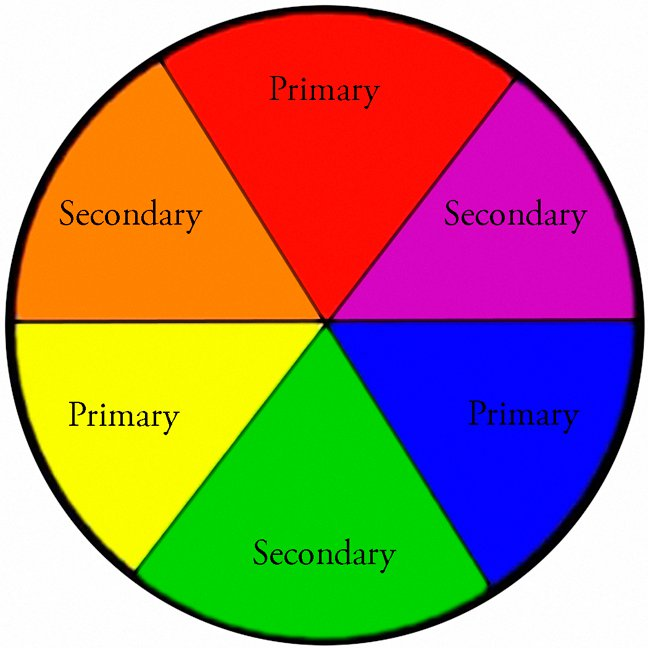
\includegraphics[width=0.55\linewidth]{colorwheel}
	
\end{frame}


\begin{frame}\frametitle{Tertiary Colors:  E.g., red-orange, blue-green, etc}
	\centering
	
	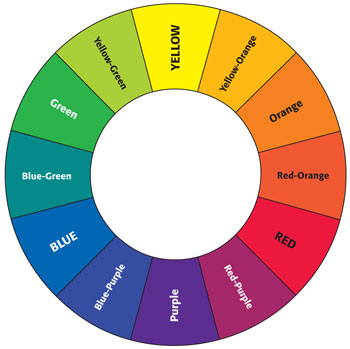
\includegraphics[width=0.77\linewidth]{colorwheel2}
	
\end{frame}



\begin{frame}\frametitle{Beyond Tertiary Colors in the Color Wheel}
	\centering
	
	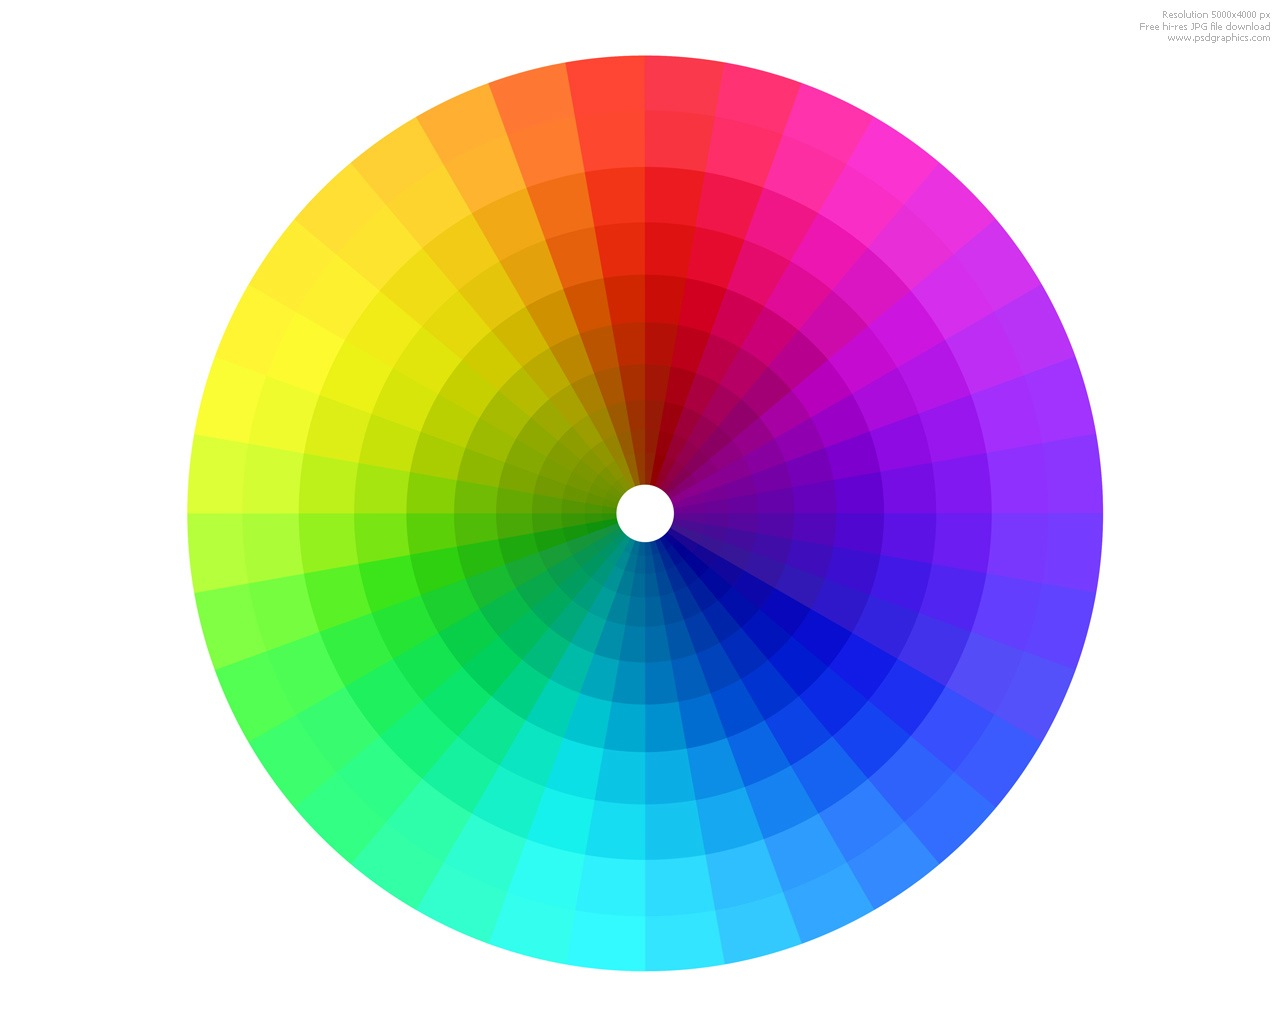
\includegraphics[width=0.87\linewidth]{colorwheel3}
	
\end{frame}



\begin{frame}\frametitle{Color varies on a continuous -- not a discrete -- scale}
	\centering
	
	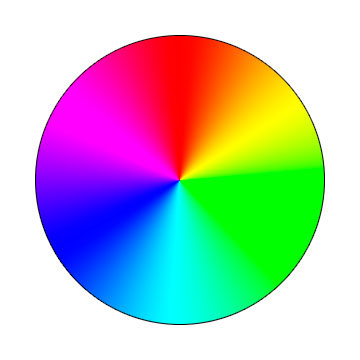
\includegraphics[width=0.8\linewidth]{colorwheel4}
	
\end{frame}



\begin{frame}\frametitle{Hue vs. Value vs. Saturation/Intensity}
	\centering
	
	\textbf{Hue}:  Name of the color\\
	\textbf{Value}:  How much white (tint)?  How much black (shading)?\\
	\textbf{Saturation/Intensity}:  The ``purity'' of the hue
	
	\vskip 0.25 cm
	
	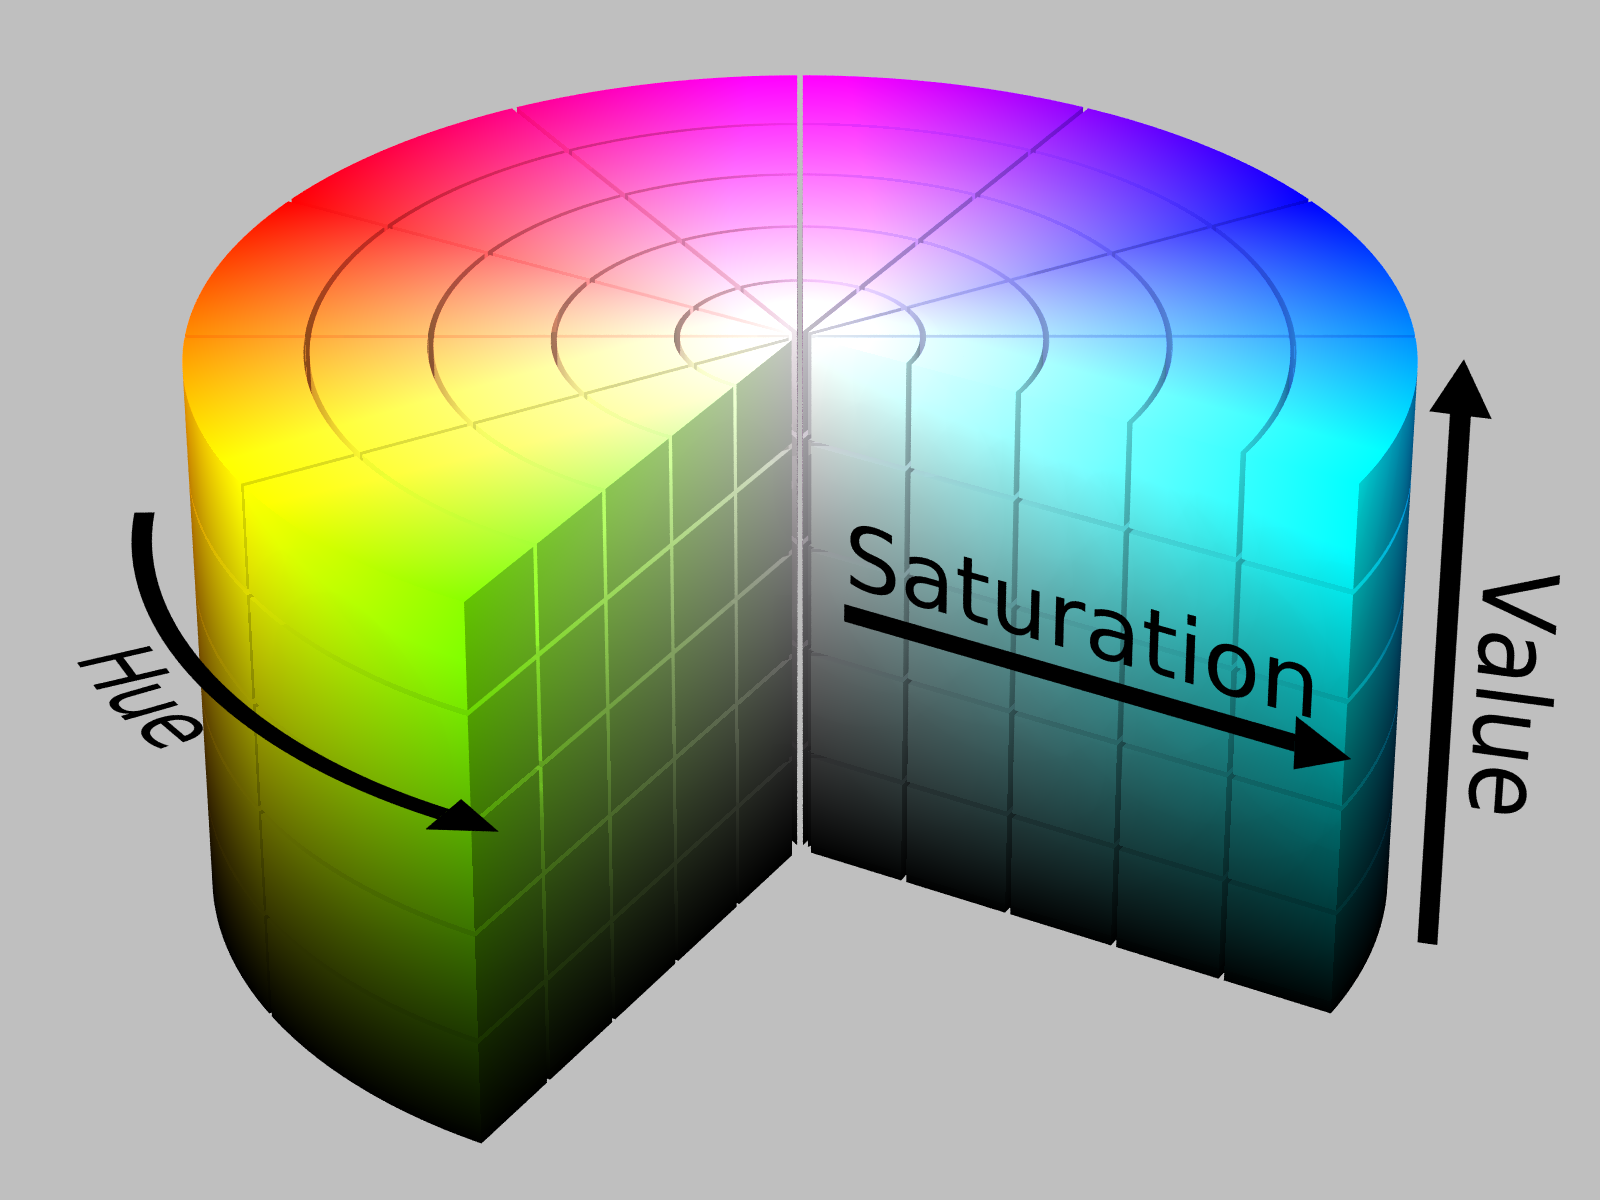
\includegraphics[width=0.77\linewidth]{colorwheel5}
	
\end{frame}




\begin{frame}\frametitle{Using Color to Represent Ideas in Data:  Warm vs. Cool}
	\centering
	
	\textbf{Warm}:  appear more active; arouse/stimulate the viewer\\
	\textbf{Cool}:  tend to recede; calm/relax the viewer
	
	\vskip 0.25 cm
	
	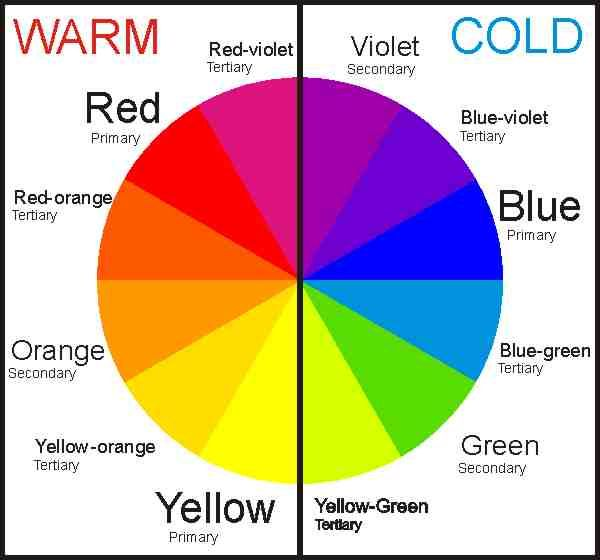
\includegraphics[width=0.66\linewidth]{warmcold}
	
\end{frame}


\begin{frame}\frametitle{Using Color Schemes to Represent Ideas in Data: \\ Analogous Colors}
	\centering
	
	\textbf{Analogous Colors}:  Appear next to each other on the color wheel
	
	\vskip 0.25 cm
	
	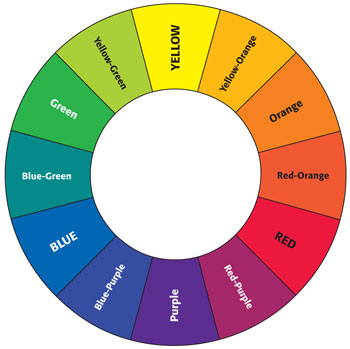
\includegraphics[width=0.55\linewidth]{colorwheel2}
	
	\textbf{Use analogous colors to represent similar groups} \\(e.g. ``Strongly agree'' vs. ``Agree'')
	
\end{frame}



\begin{frame}\frametitle{Using Color Schemes to Represent Ideas in Data:  Complementary Colors}
	\centering
	
	\textbf{Complementary Colors}:  Appear across from each other
	
	\vskip 0.25 cm
	
	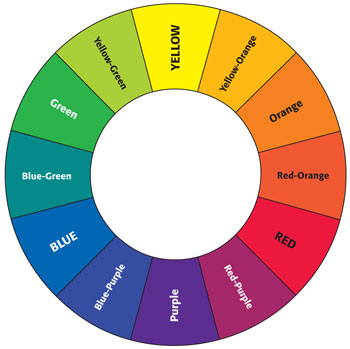
\includegraphics[width=0.55\linewidth]{colorwheel2}
	
	\textbf{Use complementary colors to represent differing groups} \\(e.g. men vs. women; ``Agree'' vs. ``Disagree'', etc)
	
\end{frame}



\begin{frame}\frametitle{Using Color Schemes to Represent Ideas in Data:  Complementary Colors}
	\centering
	
	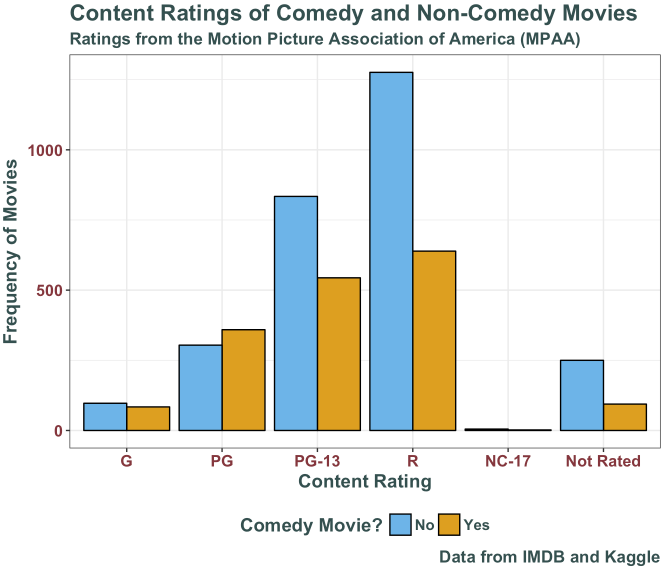
\includegraphics[width=0.81\linewidth]{labexam.png}
	
\end{frame}


\begin{frame}\frametitle{Using Color Schemes to Represent Ideas in Data:  Complementary Colors}
	\centering
	
	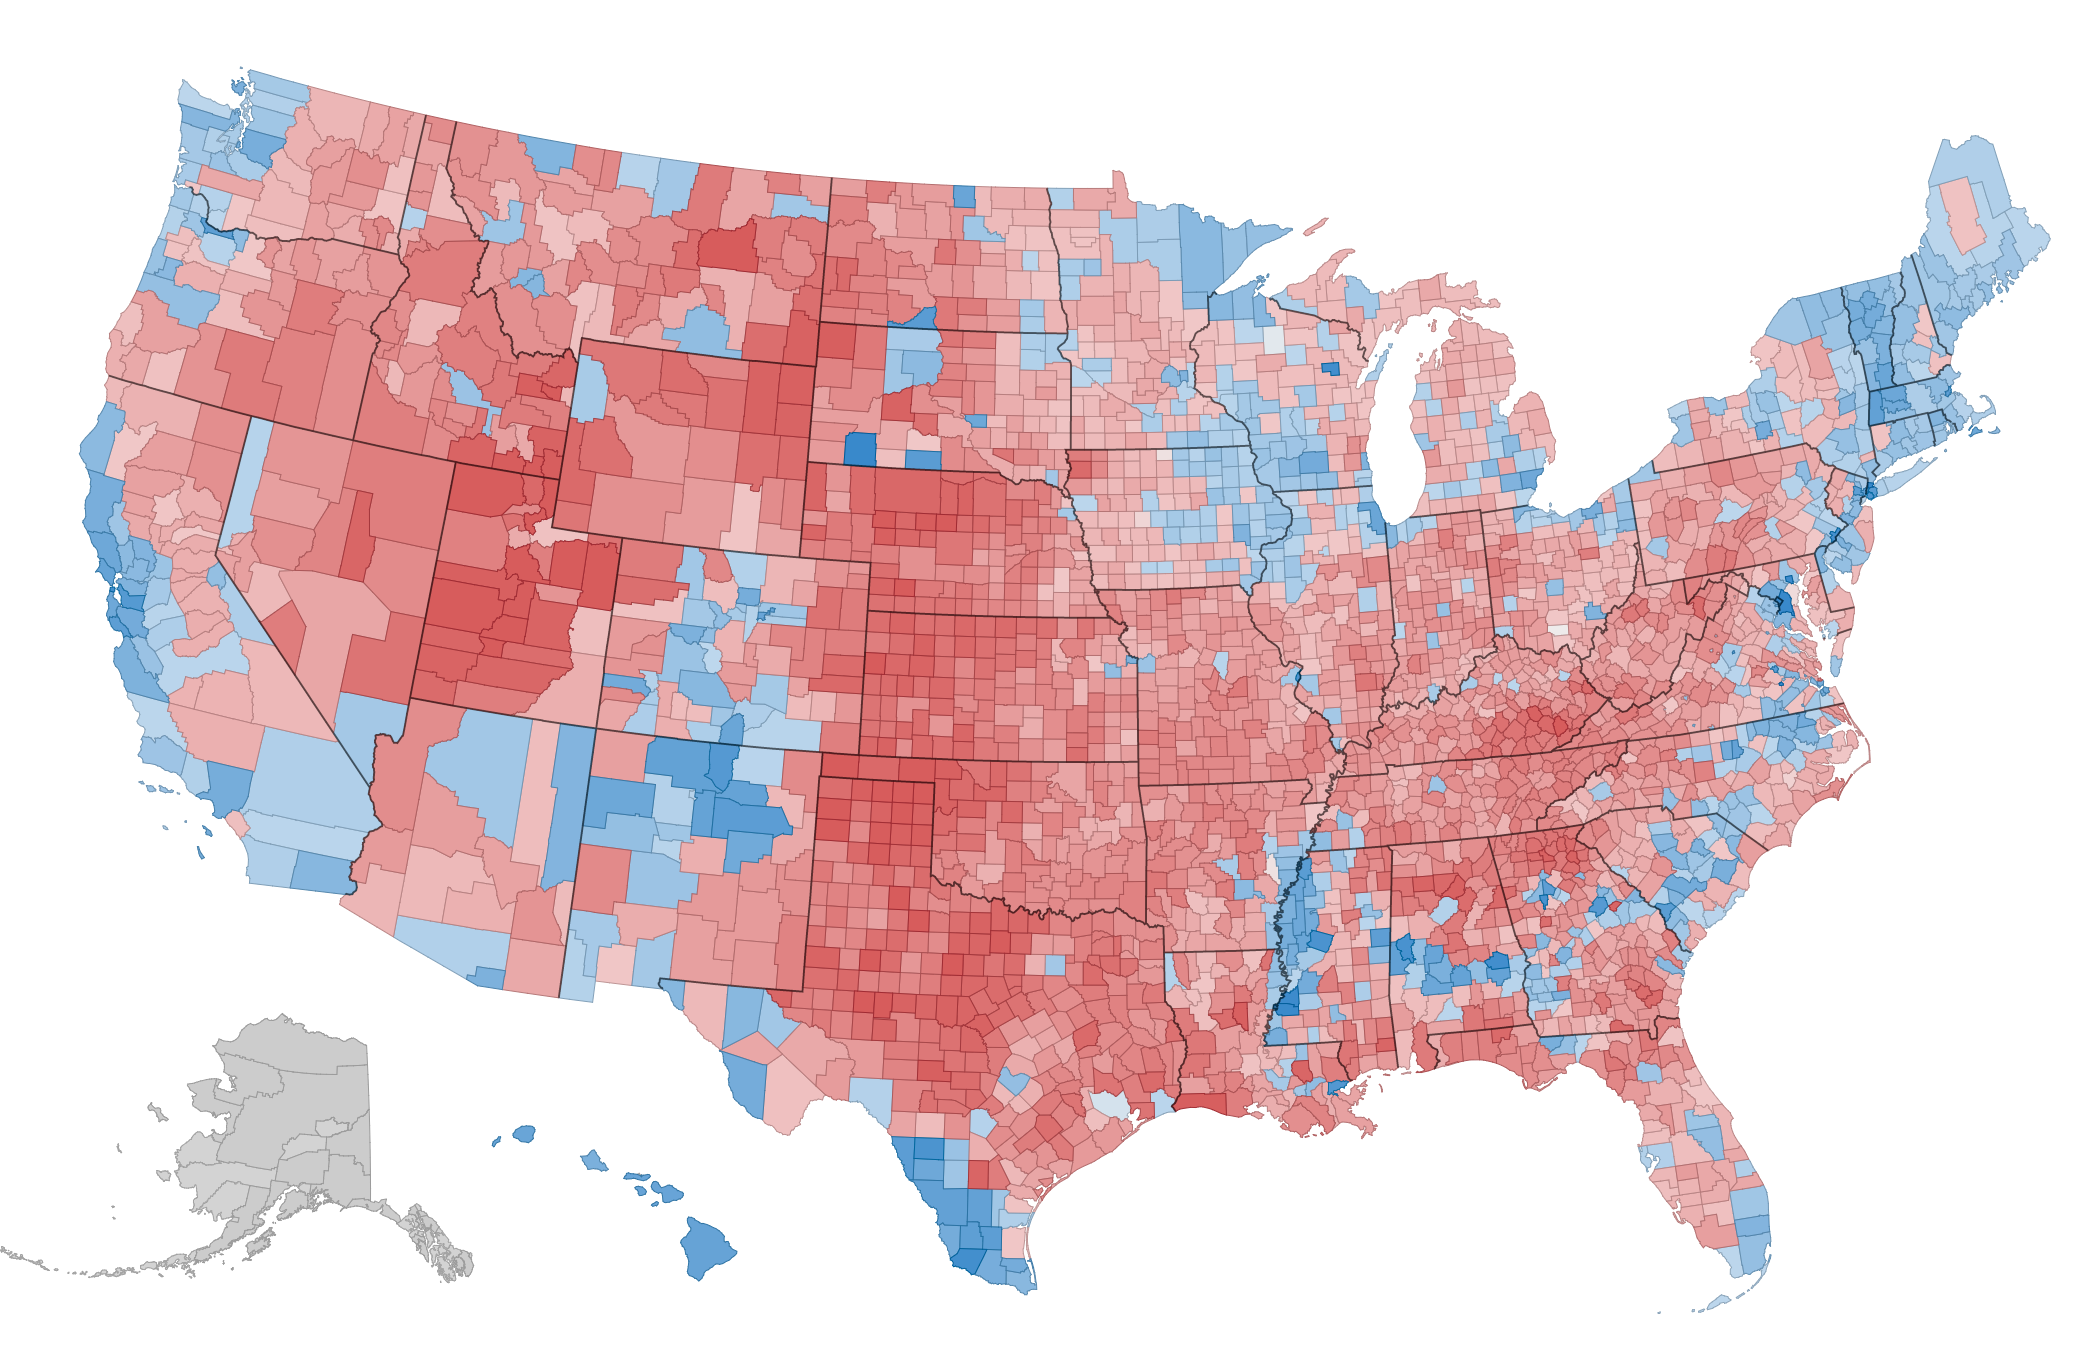
\includegraphics[width=0.81\linewidth]{election.png}
	
\end{frame}


\begin{frame}\frametitle{Using Color Schemes to Represent Ideas in Data:  Complementary Colors}
	\centering
	
	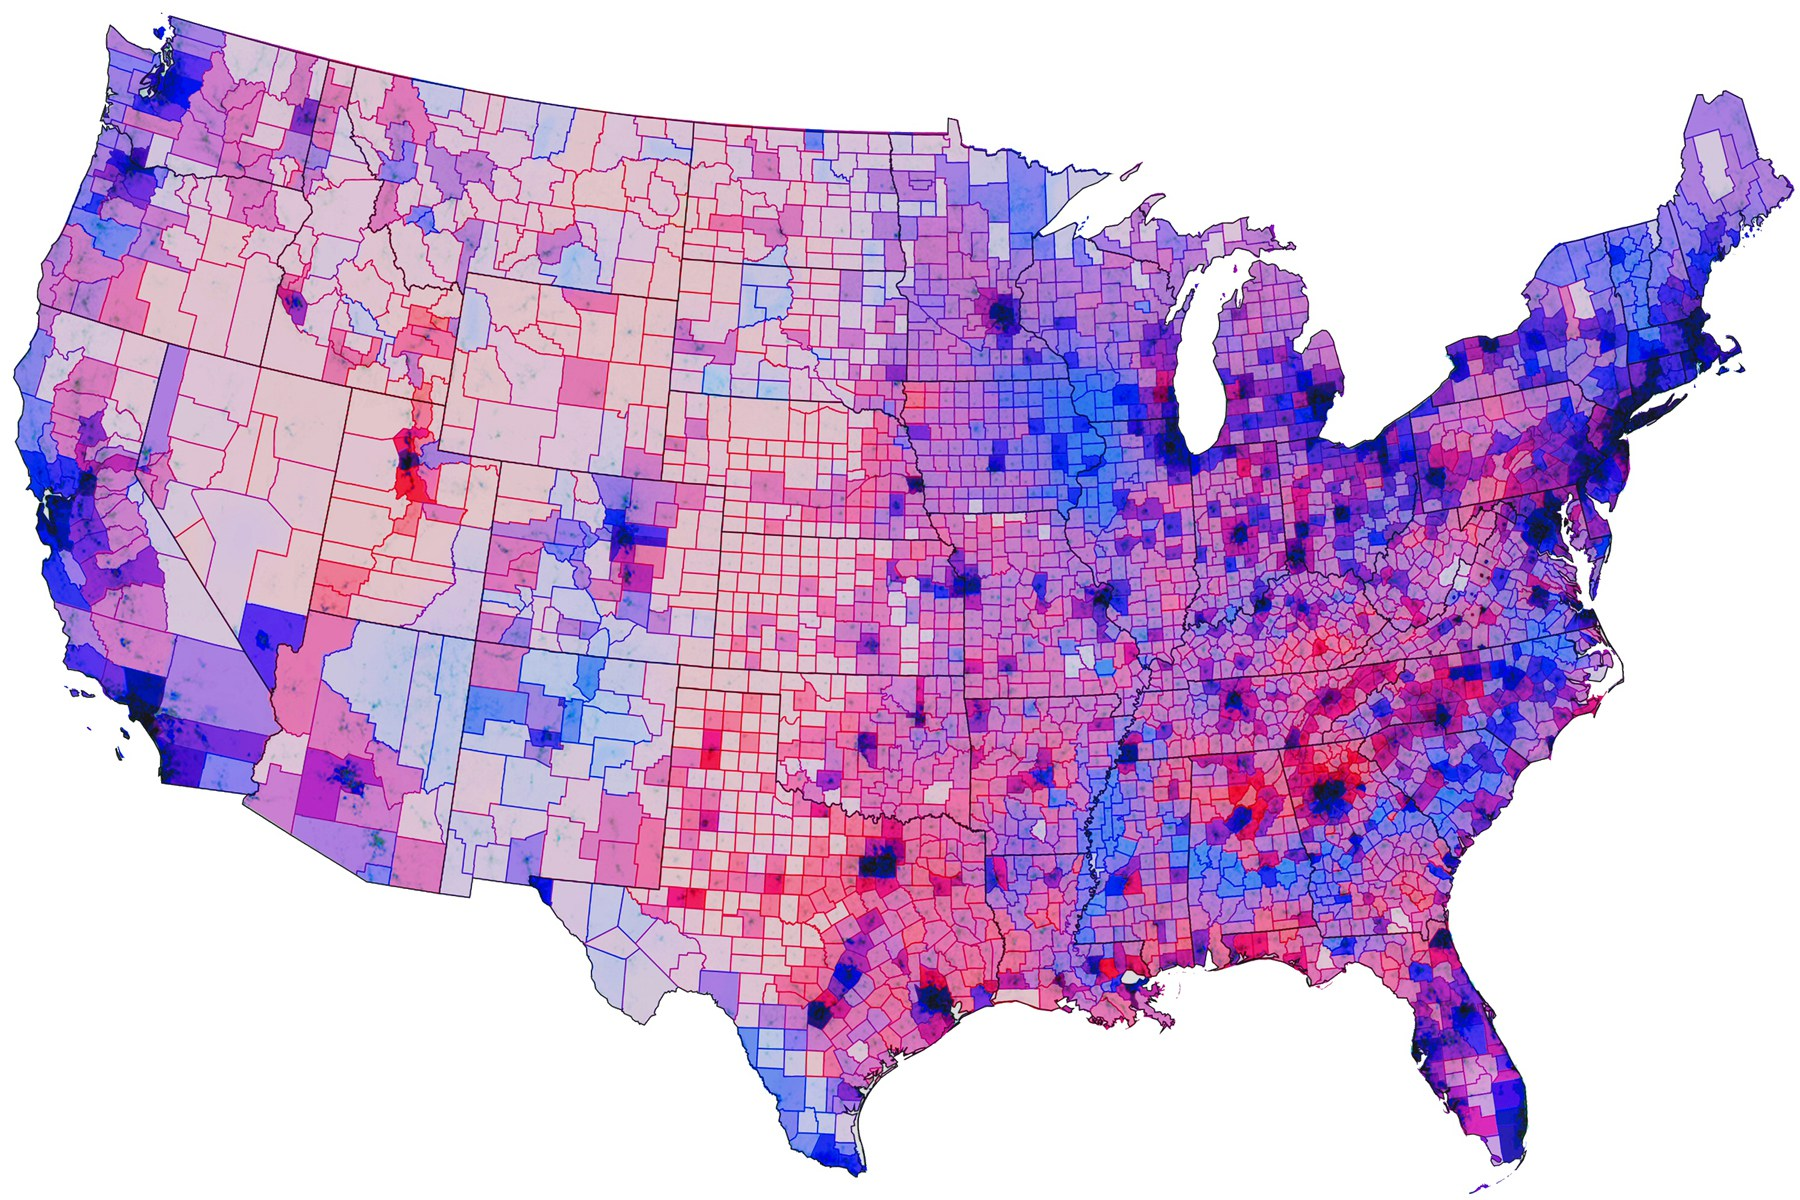
\includegraphics[width=0.81\linewidth]{election.jpg}
	
\end{frame}

\begin{frame}\frametitle{Using Color Schemes to Represent Ideas in Data:  Complementary Colors}
	\centering
	
	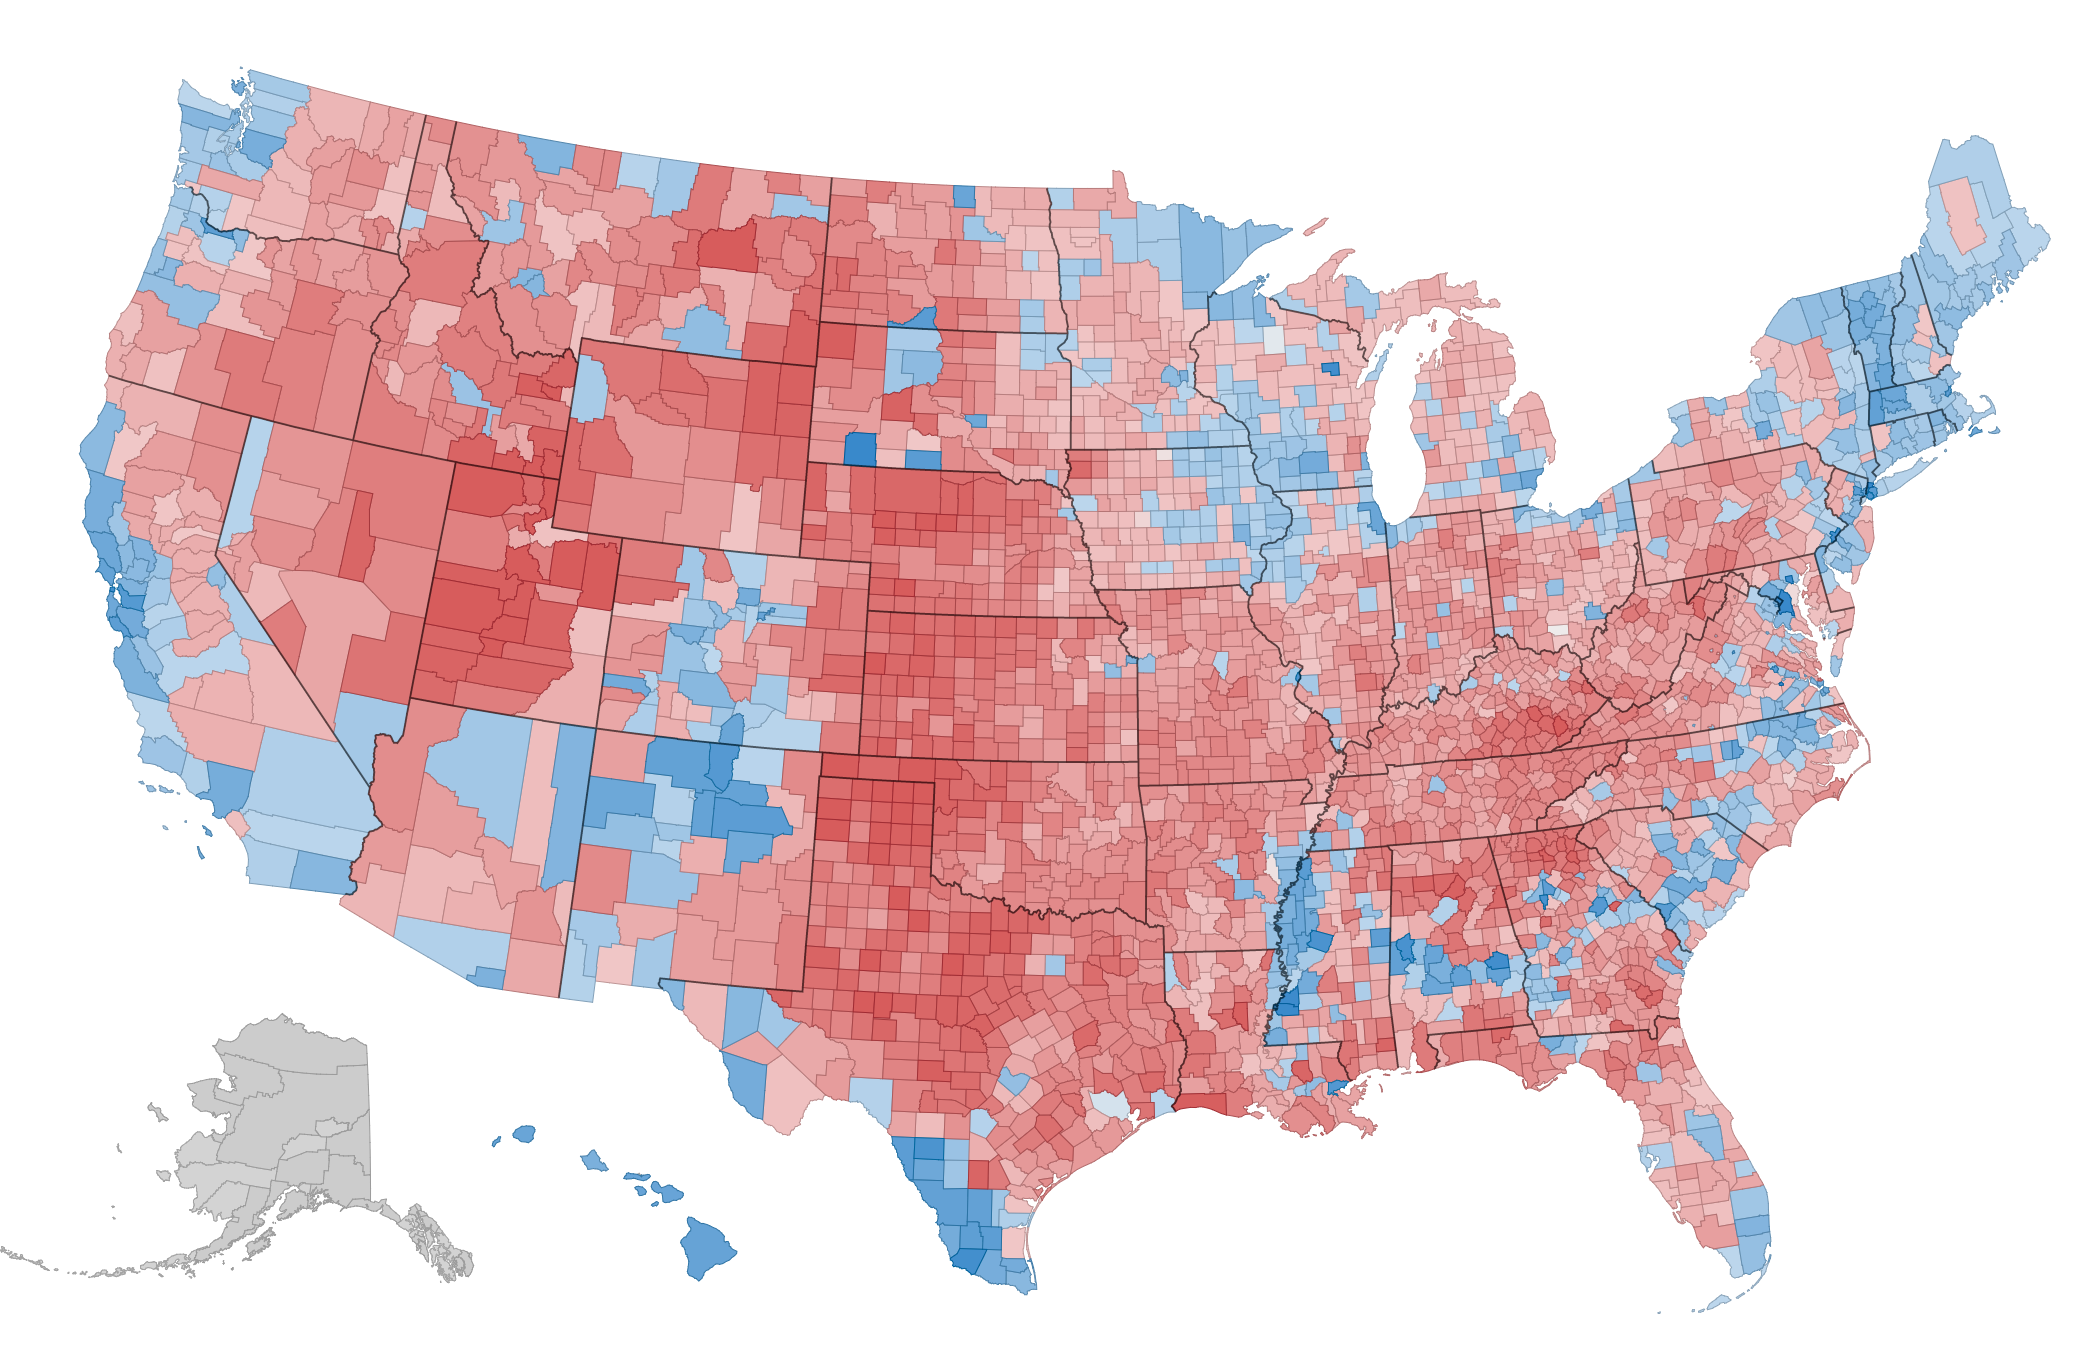
\includegraphics[width=0.51\linewidth]{election.png}\\
	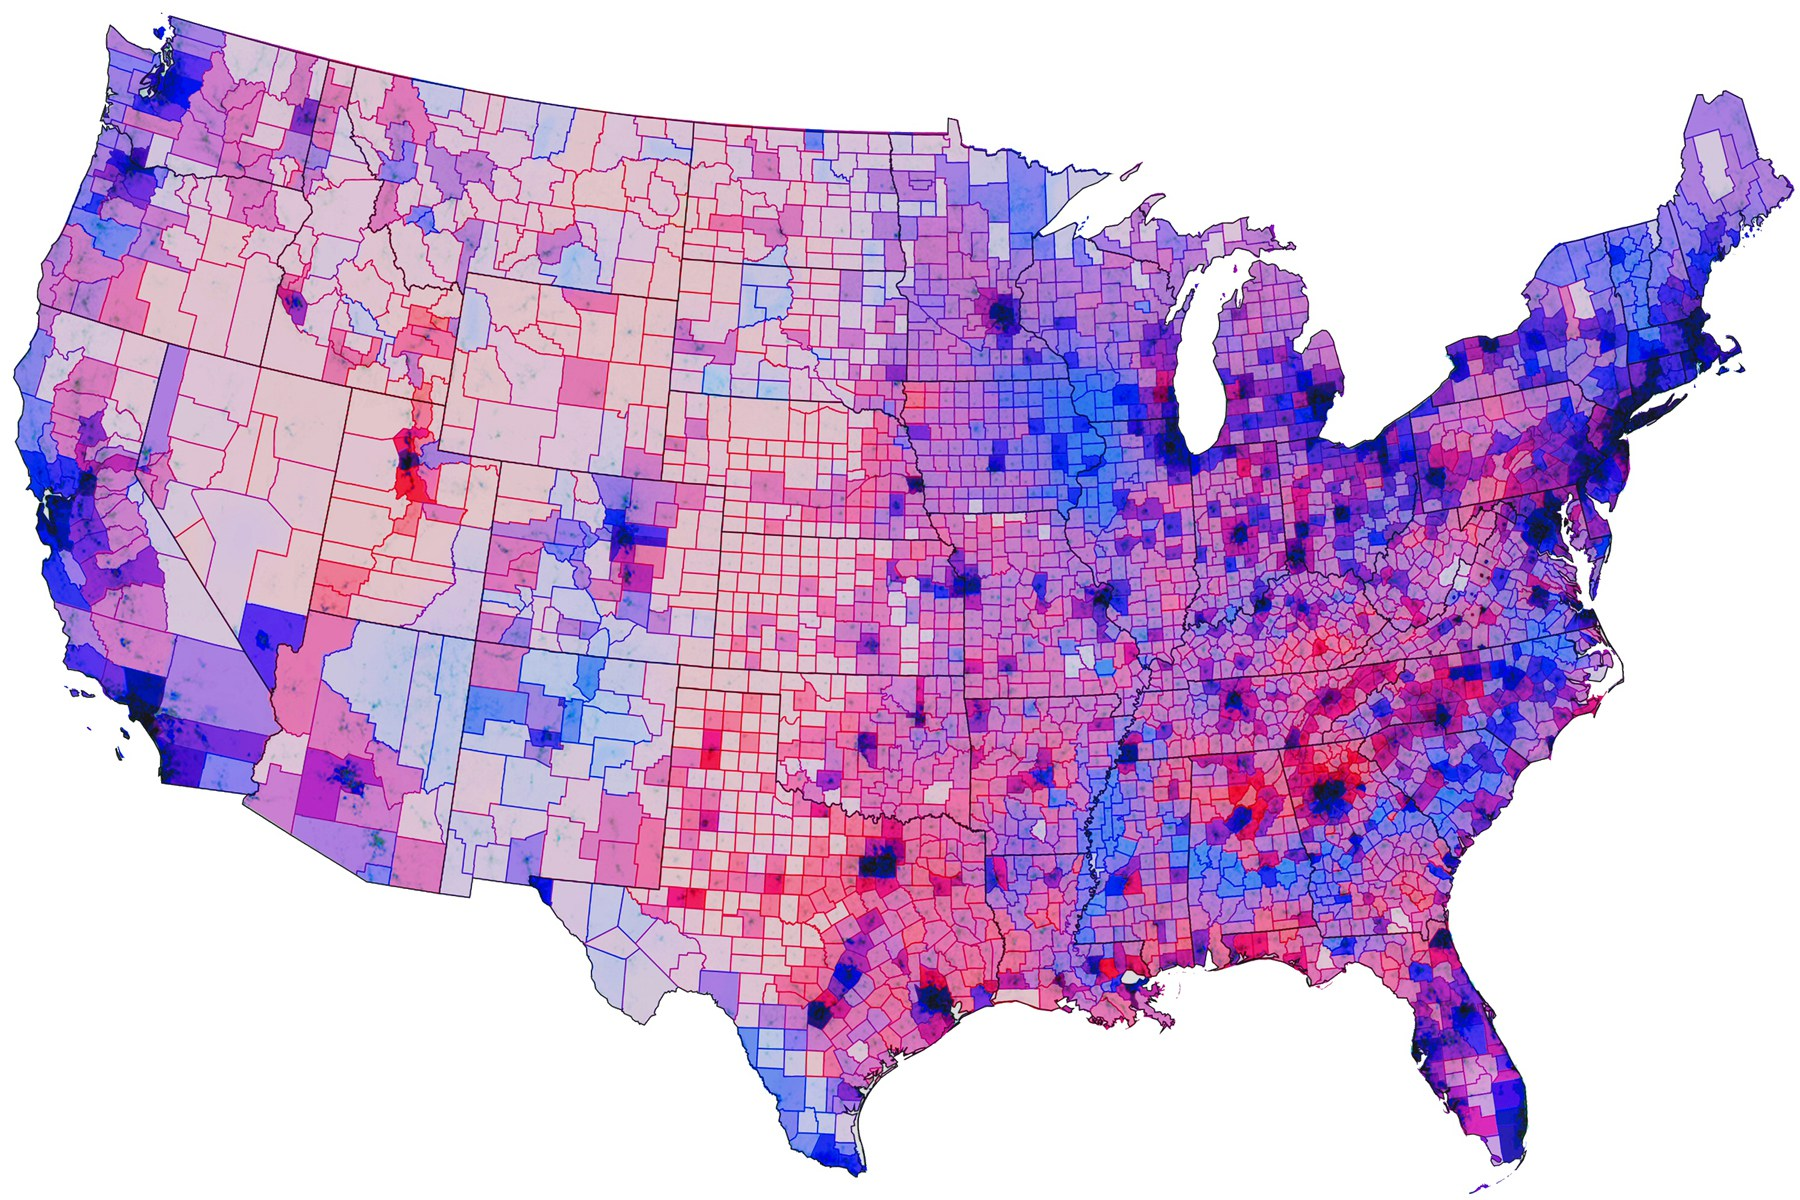
\includegraphics[width=0.51\linewidth]{election.jpg}
	
\end{frame}


\begin{frame}\frametitle{Using Color Schemes in Art: Analogous Colors}
	\centering
	
	Vincent Van Gogh, \emph{Wheat Fields After The Rain} (1890)\\
	
	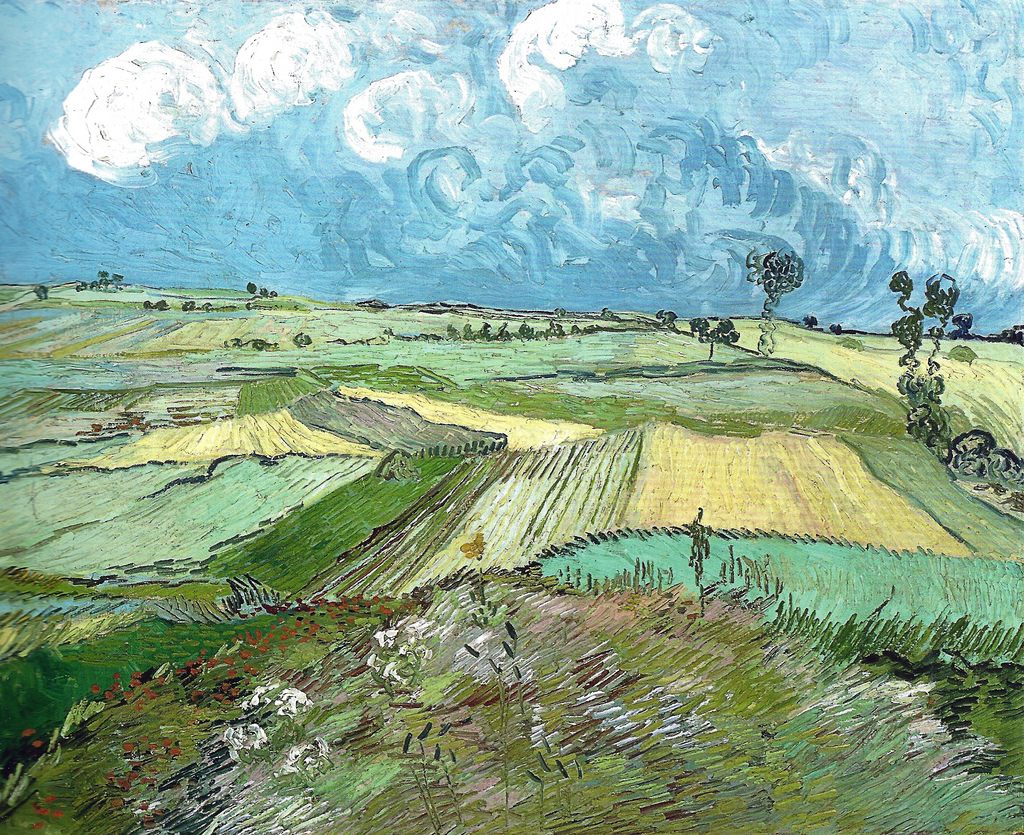
\includegraphics[width=0.87\linewidth]{vangogh}
	
\end{frame}


\begin{frame}\frametitle{Using Color Schemes in Art: Complementary Colors}
	\centering
	
	Paul Signac, \emph{Place des Lices, St. Tropez} (1893)\\
	
	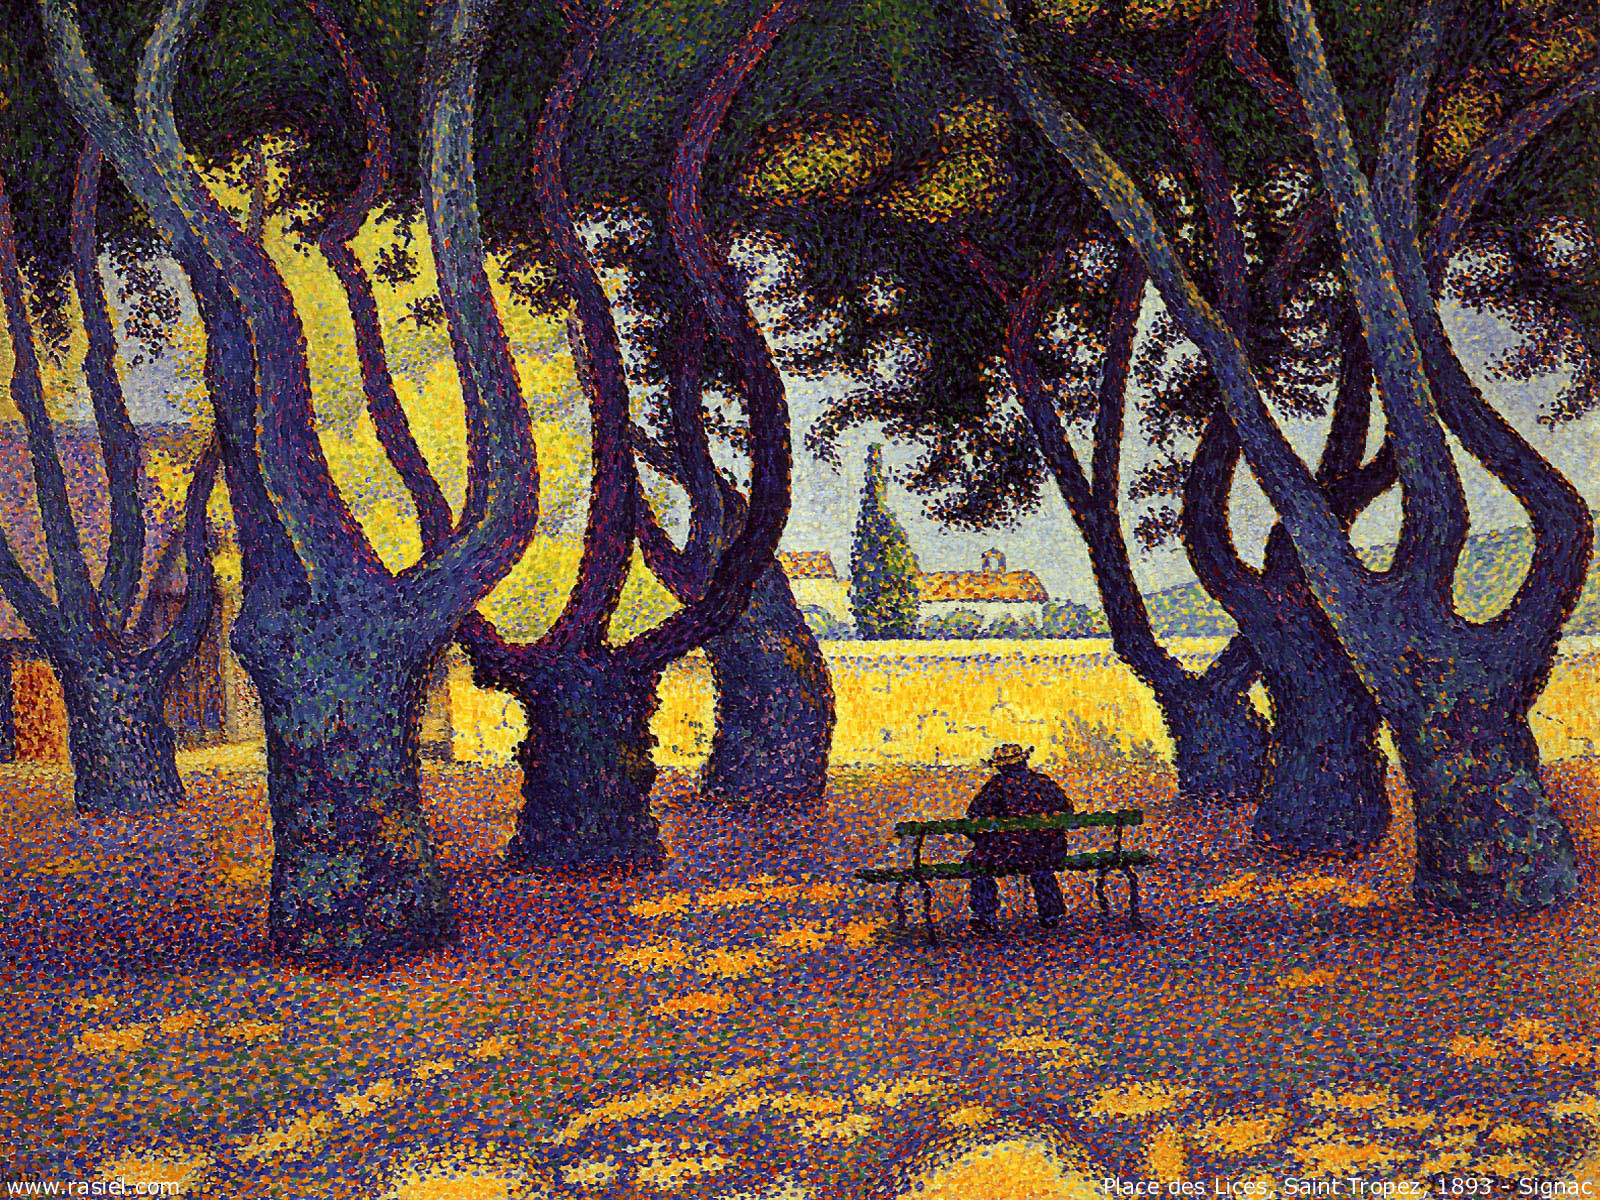
\includegraphics[width=0.95\linewidth]{signac}
	
\end{frame}


\begin{frame}\frametitle{Using Color Schemes in Art: Complementary Colors}
	\centering
	
	Jasper Johns, \emph{Flag} (1969)\\
	
	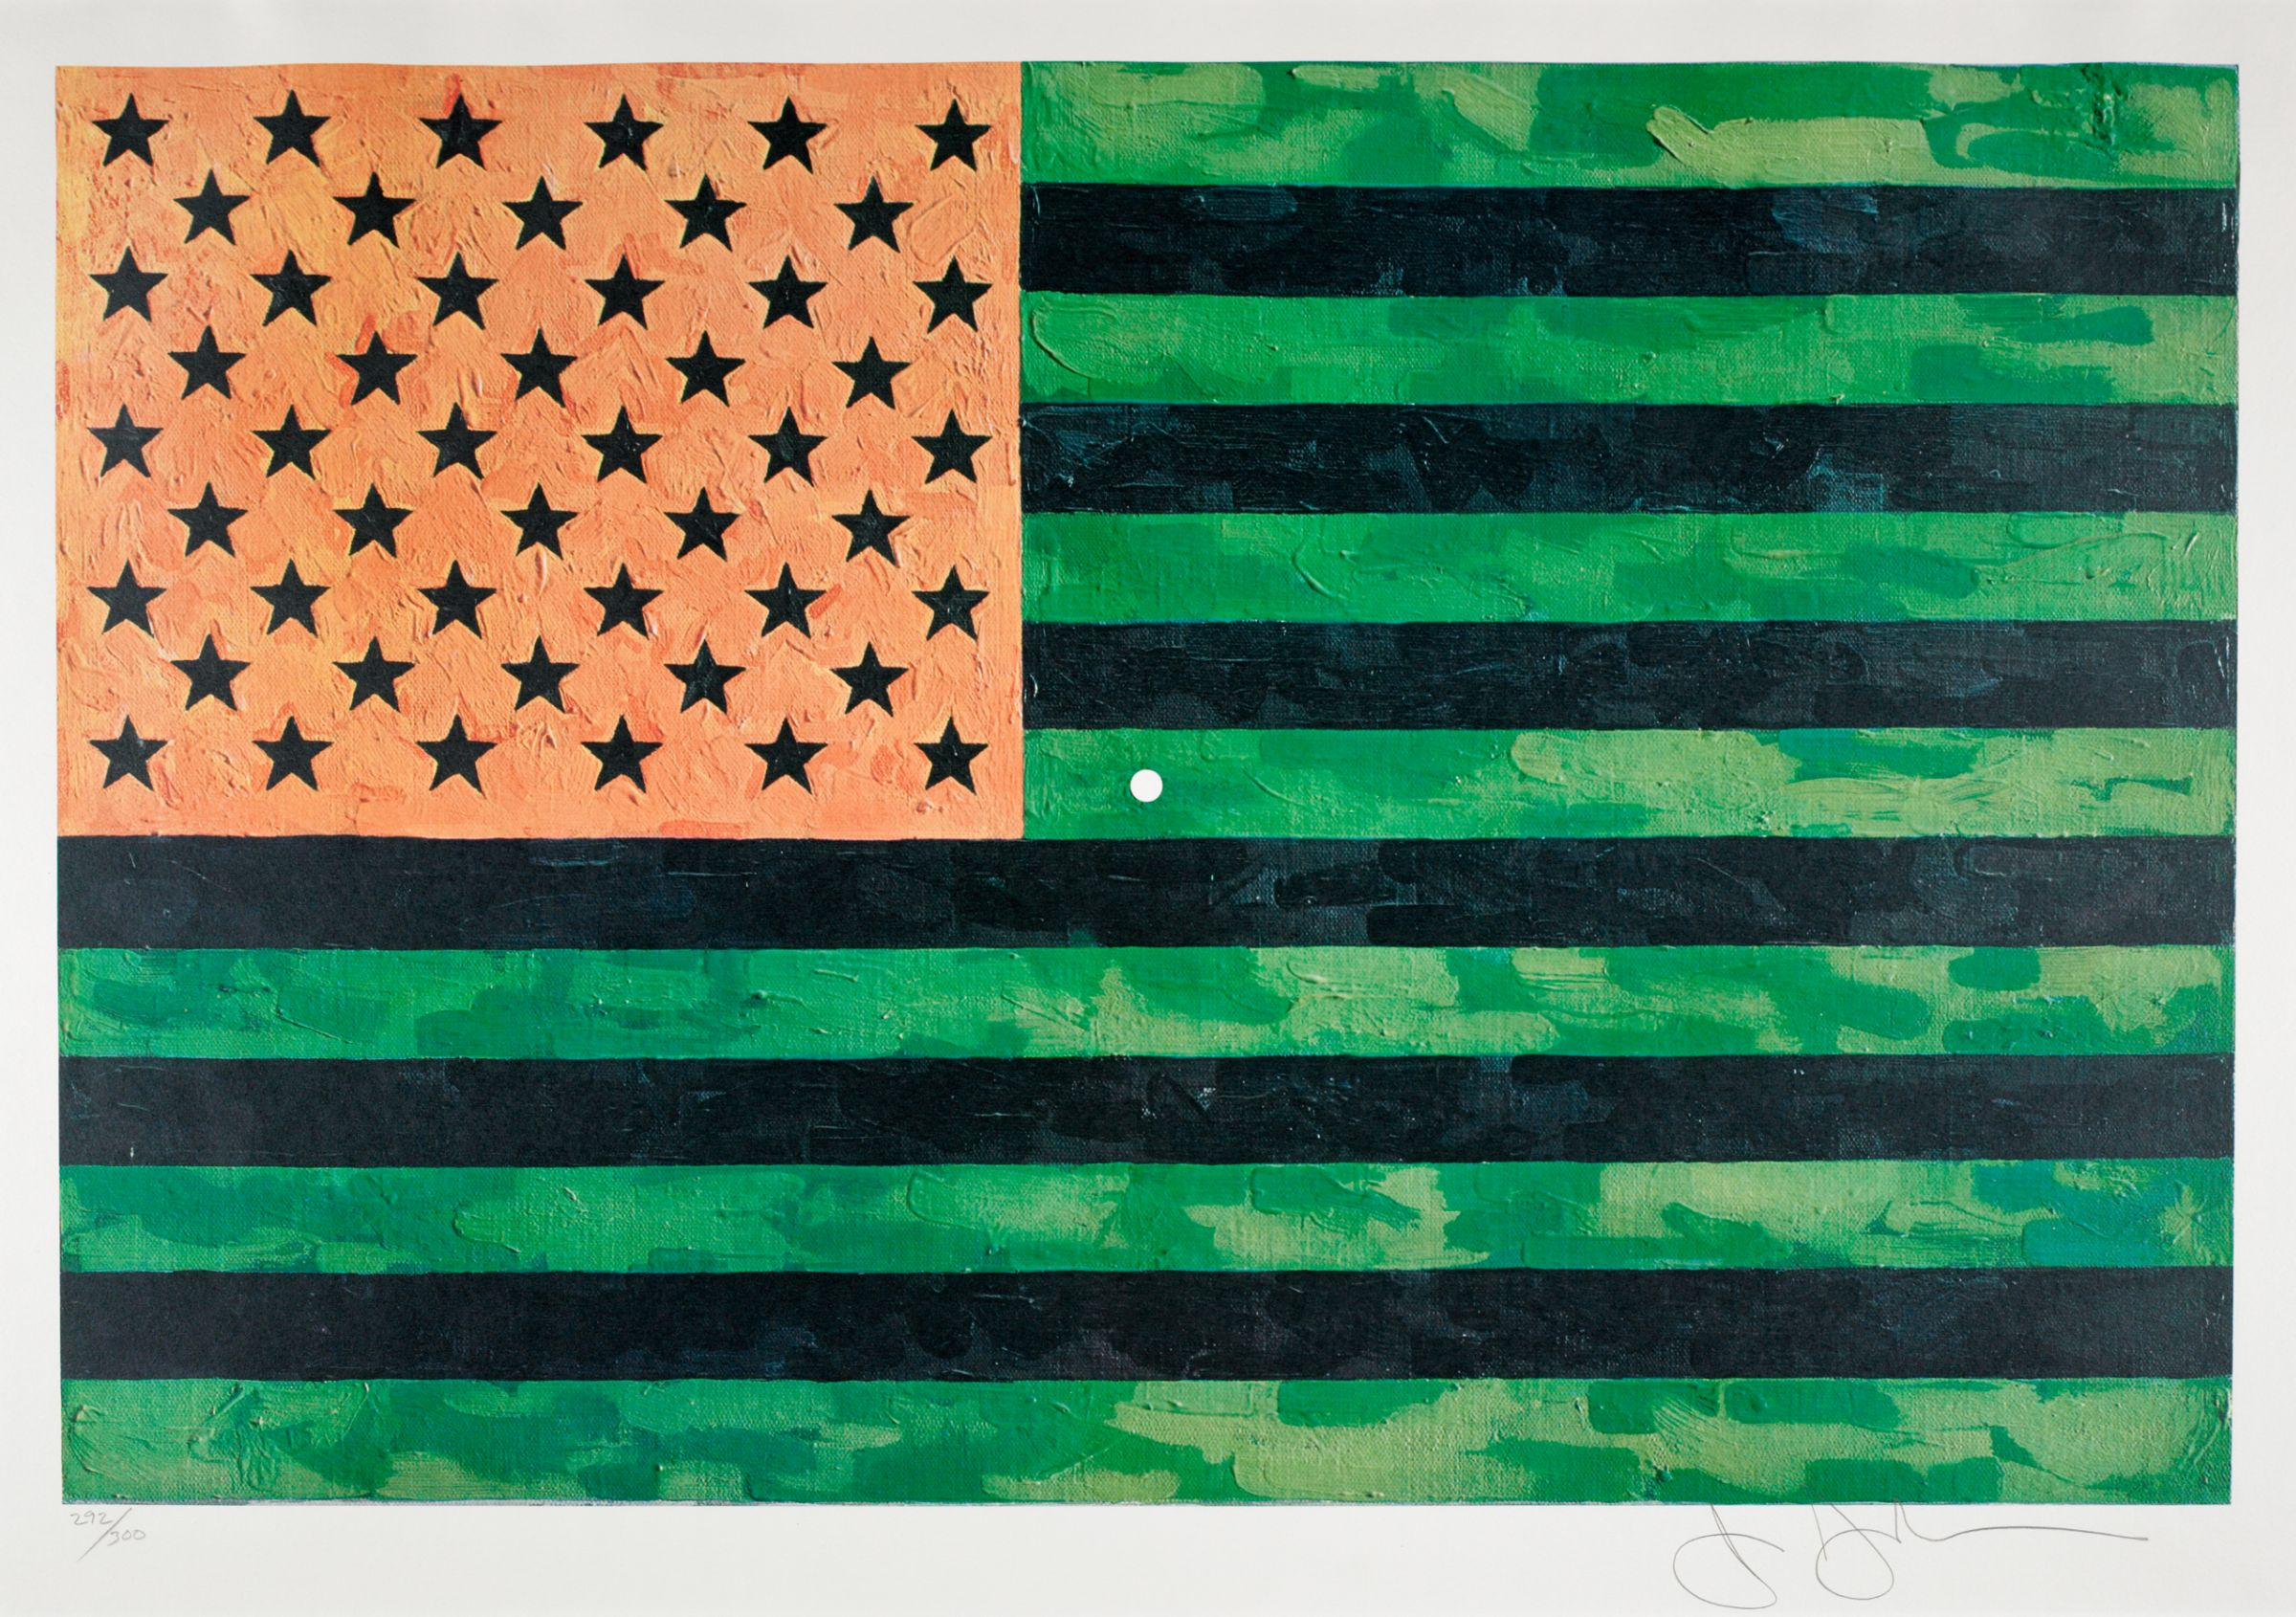
\includegraphics[width=\linewidth]{flag}
	
\end{frame}



\begin{frame}\frametitle{Color Blindness}
	\centering
	
	\textbf{About 8\% of men are color blind}\\
	About 0.5\% of women are color blind
	
	\vskip 0.15 cm
	
	Most common form of color blindness:  Deuteranopia (``red-green'')
	
	\vskip 0.15 cm
	
	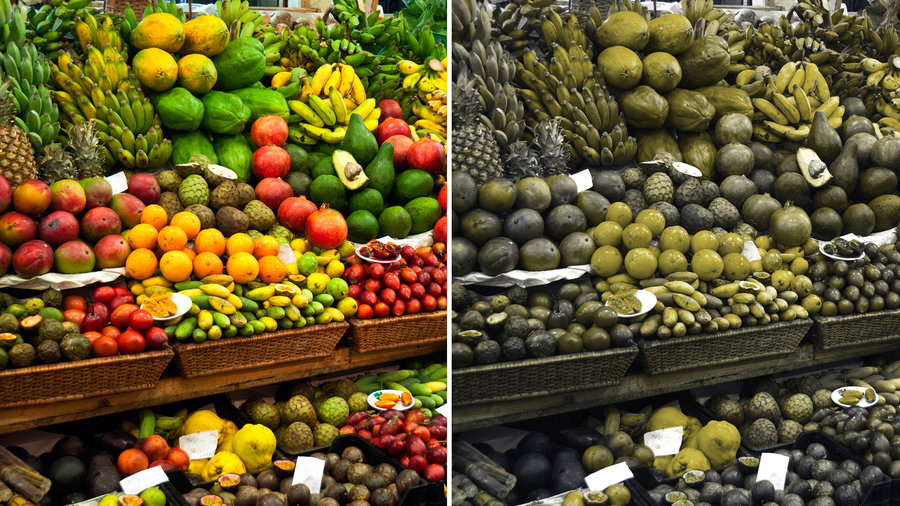
\includegraphics[width=0.66\linewidth]{redgreen}\\
	
	\vskip 0.15 cm
	
	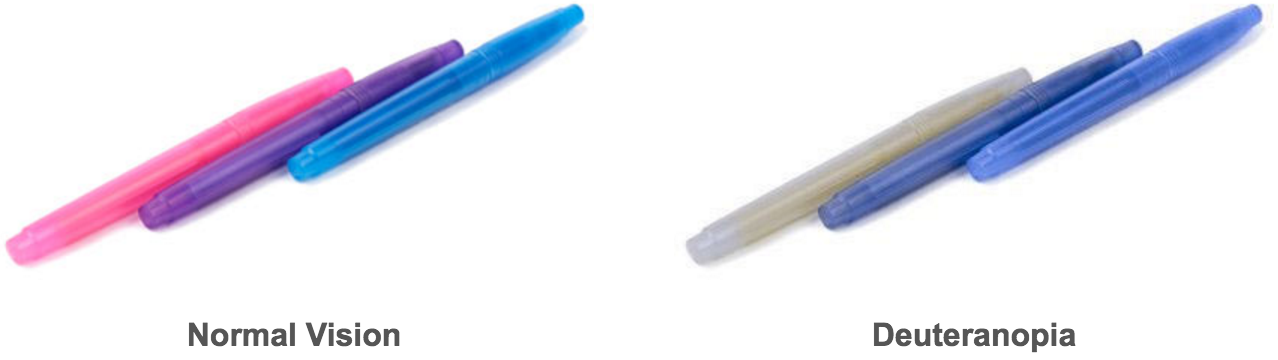
\includegraphics[width=0.77\linewidth]{redgreen2}
	
\end{frame}



\begin{frame}\frametitle{RGB Colors}
	\small
	\centering
	
	\textbf{RGB}:  On computers, colors can be generated by \\varying the amount of red, green, and blue light
	
	
	\vskip 0.5 cm
	
	Represent RGB as 3-D space:  Red $\in [0,1]$, Green $\in [0,1]$, Blue $\in [0,1]$
	
	\vskip 0.25 cm
	
	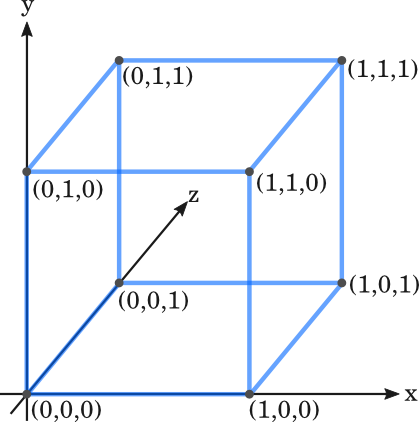
\includegraphics[width=0.55\linewidth]{xyzcube}
	
\end{frame}



\begin{frame}\frametitle{The Color Cube}
	\small
	\centering
	
	Represent RGB as 3-D space:  Red $\in [0,1]$, Green $\in [0,1]$, Blue $\in [0,1]$
	
	\vskip -0.1 cm
	
	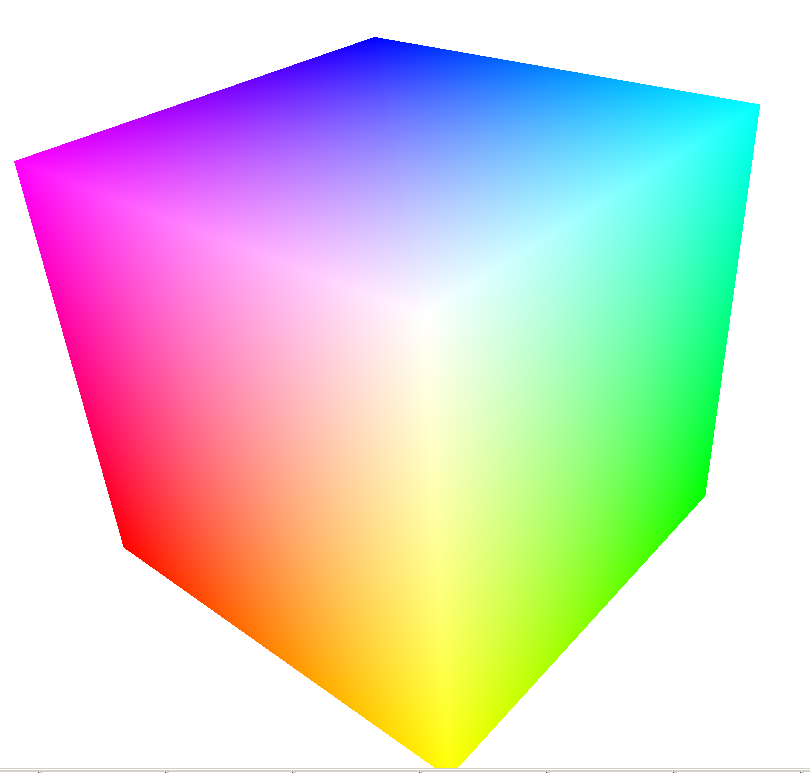
\includegraphics[width=0.28\linewidth]{colorcube}	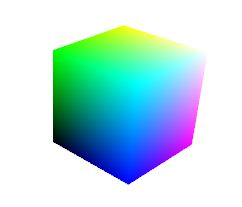
\includegraphics[width=0.38\linewidth]{colorcube2}	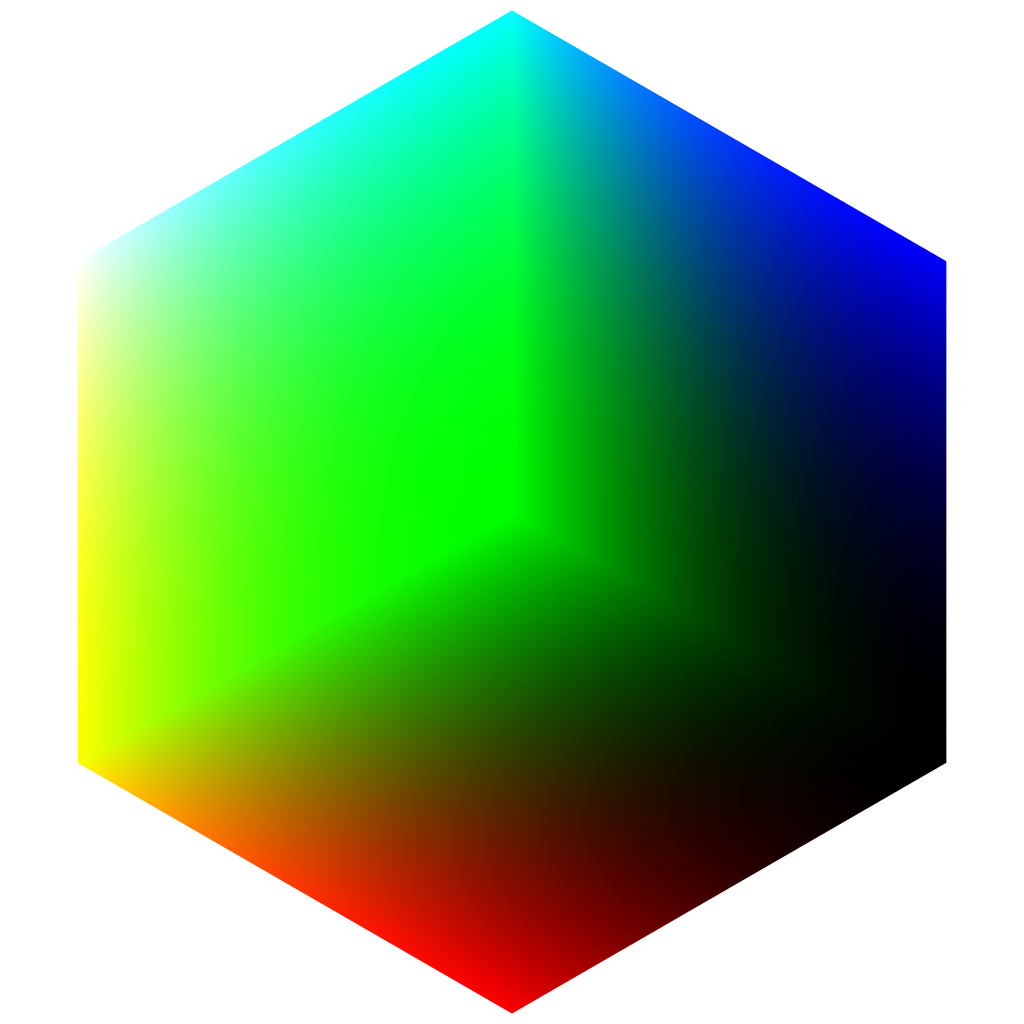
\includegraphics[width=0.28\linewidth]{colorcube3}
	
	\vskip 0.25 cm
	
	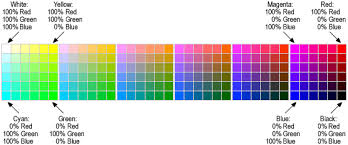
\includegraphics[width=0.9\linewidth]{colorcube5}
\end{frame}




\end{document}
